\documentclass{article}
\usepackage[utf8]{inputenc}
\usepackage[spanish]{babel}
\usepackage{graphicx}
\usepackage{anysize}
\usepackage{fancyhdr} 
\usepackage[export]{adjustbox}
\usepackage{titlesec}
\usepackage{enumitem}
\usepackage{listings}
\usepackage{xcolor}
\usepackage{array}
\usepackage{longtable}
\usepackage{multicol}
% \usepackage{hyperref}
% \usepackage{float}
% \usepackage{tabu}

% Izquierda, derecha, arriba, abajo
\marginsize{2cm}{2cm}{1.2cm}{1.5cm} 
\renewcommand{\familydefault}{\sfdefault}
\decimalpoint%

\graphicspath{{assets/}{tema04-ej-prac-01.assets/}}

\setlength{\parindent}{0in}
\titleformat*{\section}{\large\bfseries}

% Para insert código
\definecolor{codegreen}{rgb}{0,0.6,0}
\definecolor{codegray}{rgb}{0.5,0.5,0.5}
\definecolor{codepurple}{rgb}{0.58,0,0.82}
\definecolor{backcolour}{rgb}{1,1,1}

\usepackage{textcomp}
\lstset{upquote=true}
\lstdefinestyle{mystyle}{
    backgroundcolor=\color{backcolour},   
    commentstyle=\color{codegreen},
    keywordstyle=\color{magenta},
    numberstyle=\tiny\color{codegray},
    stringstyle=\color{codepurple},
    basicstyle=\ttfamily\footnotesize,
    breakatwhitespace=false,         
    breaklines=true,                 
    captionpos=b,                    
    keepspaces=true,                 
    % numbers=left,                    
    % numbersep=5pt,                  
    showspaces=false,                
    showstringspaces=false,
    showtabs=false,                  
    tabsize=2
}

\lstset{style=mystyle}

\newcommand{\materia}{BDA}
\newcommand{\clave}{2929}
\newcommand{\profesor}{Ing. Rodriguez Campos \textsc{Jorge Alberto}}
\newcommand{\grupo}{1}
\newcommand{\semestre}{2021-1}

\newcommand{\alumno}{Francisco Pablo \textsc{Rodrigo}}

\newcommand{\actividad}{Tema 04 \\ Ejercicio práctico 01}
\newcommand{\titulo}{Administración de parámetros}

\newcommand{\fechaEntrega}{16 de noviembre de 2020}

%%%%%%%%%%%%%%%%%%%% ENCABEZADO %%%%%%%%%%%%%%%%%%%%%%%%%%%%
\pagestyle{fancy}
\fancyhf{}
\renewcommand{\headrulewidth}{0pt}
\fancyhead[R]{% Left header
    {\renewcommand*{\arraystretch}{1}
    \begin{tabular}{l}
        \materia \\ 
        \actividad%
    \end{tabular}}
    \,% Space
    \rule[-1.75\baselineskip]{0pt}{0pt}
    % Strut to ensure a 1/4 \baselineskip between image and header rule
    
\includegraphics[height=3\baselineskip,valign=c]{unam}
}
\setlength{\headsep}{0.3in}


\begin{document}
%%%%%%%%%%%%%%%%%%% DATOS PORTADA %%%%%%%%%%%%%%%%%%%%%%%%
\thispagestyle{empty}
\begin{minipage}[t][5cm][t]{0.2\linewidth}
    
\includegraphics[width=2.5cm]{unam.jpg}
    \vspace{10cm}

    
\includegraphics[width=2.5cm]{fiblack}
\end{minipage}
\begin{minipage}[t]{0.7\linewidth}
    \vspace{-2.5cm}
    \LARGE{\textbf{Universidad Nacional Autónoma de México}}\\
    \Large{\textbf{Facultad de Ingeniería}} \\

    \large{\semestre}\\[2cm]

    \large{\textbf{\materia (\clave)}}\\
    \large{\textbf{Gpo: 1}}\\[5mm]
    \large{\textbf{Profesor:} \profesor}\\ [1.5cm]
    \begin{center}
        \LARGE{\textbf{\actividad}}\\
        \LARGE{\textbf{\titulo}}\\
    \end{center}

    \vspace{3.3cm}

    \large{\textbf{Alumno:} \alumno} \\[1.5cm]

    \begin{flushright}
        \fechaEntrega%
    \end{flushright}
\end{minipage}

\newpage
%%%%%%%%%%%%%%%%%%% CONTENIDO %%%%%%%%%%%%%%%%%%%%%%%%

\section*{Objetivos}
Conocer y familiarizarse con las principales vistas y parámetros de la base de 
datos que muestran o contienen información relevante acerca del uso
de las diferentes áreas de la SGA.

\section*{C1. Código del script \texttt{s-01-sga-components.sql}}

\lstinputlisting[language=SQL]{tema04-ej-prac-01-codigo/s-01-sga-components.sql}

\section*{C2. Respuesta del inciso E}
\textbf{¿Qué posibles tipos de operaciones se le pueden aplicar 
  a los componentes de la SGA? Describir brevemente cada tipo.}

Las operaciones que se pueden aplicar a la memoria son las siguientes:
\begin{itemize}
    \item \textbf{STATIC}: La memoria no esta en uso
    \item \textbf{INITIALZING}: La memoria esta un uso
    \item \textbf{DISABLED}: La memoria ha sido deshabilitada
    \item \textbf{GROW}: Se expandió la memoria designada
    \item \textbf{SHRINK}: Se encogió la memoria designada
    \item \textbf{SHRINK\_CANCEL}: Se canceló el proceso de encogimiento de la
    memoria designada
\end{itemize}

\section*{C3. Mostrar el contenido de cada una de las tablas t0* creadas en 
este ejercicio.}

% \vspace{2cm}
\textbf{Tabla 01} \\
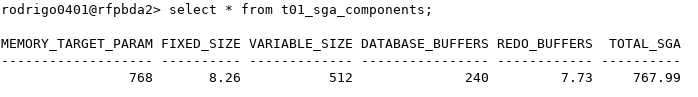
\includegraphics[width=0.8\linewidth]{t01} \\[5mm]
\newpage
\textbf{Tabla 02} \\
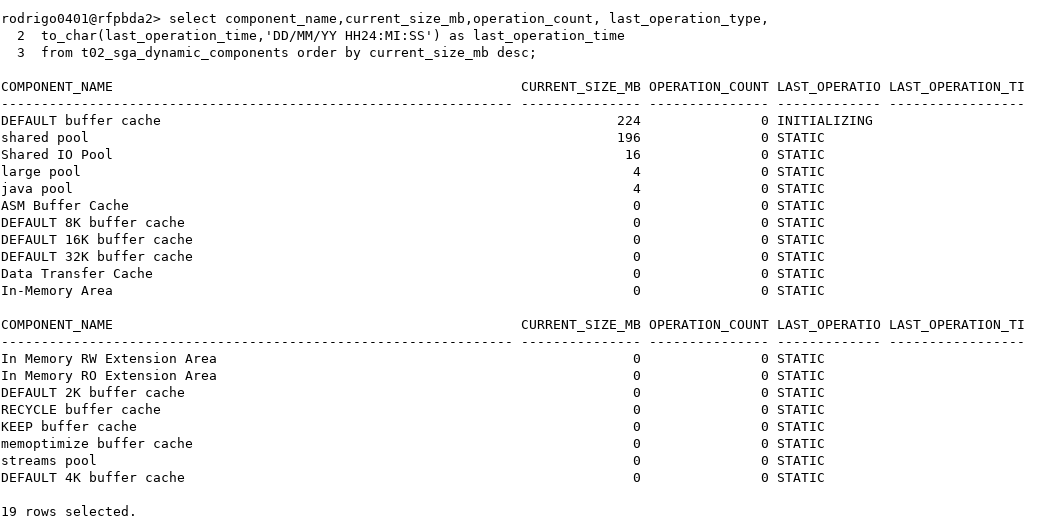
\includegraphics[width=\linewidth]{t02} \\[5mm]
\textbf{Tabla 03} \\
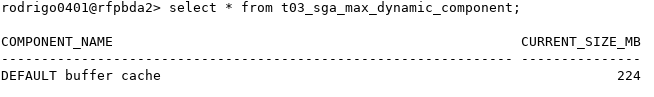
\includegraphics[width=0.8\linewidth]{t03} \\[5mm]
\textbf{Tabla 04} \\
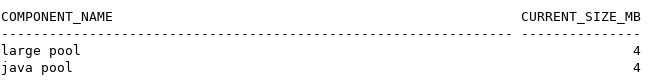
\includegraphics[width=0.8\linewidth]{t04} \\[5mm]
\textbf{Tabla 05} \\
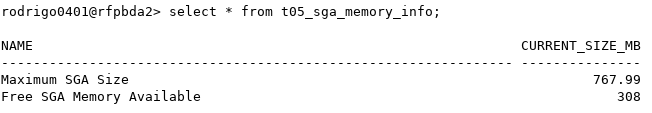
\includegraphics[width=0.8\linewidth]{t05} \\[5mm]
\textbf{Tabla 06} \\
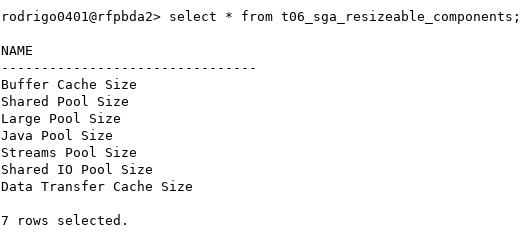
\includegraphics[width=0.6\linewidth]{t06} \\[5mm]

\section*{Comentarios y conclusiones}

En este ejercicio pudimos poner en práctica lo aprendido en el tema 4. Debido a 
que pudimos ver de manera más `tangible' el tamaño y el tipo de componentes
que presenta la sga. Así mismo, pudimos apreciar la existencia de los 
componentes estáticos y dinámicos. Para estos últimos recordemos que el dbms
puede modificar el tamaño en memoria de estos elementos de acuerdo a sus 
necesidades. 

\renewcommand\refname{Bibliografía y referencias}
\begin{thebibliography}{99}
    \bibitem{burleson} Burleson Consulting. \textit{Oracle tips } en 
    \texttt{http://www.dba-oracle.com/oracle\_news/}
    \bibitem{oracle} Oracle Help Center. \textit{v\$sga\_dynamic\_components}. 
    Database Reference en 
    \texttt{https://docs.oracle.com/
    cd/E57185\_01/ESBTR/maxl\_commands\_spool.html}
    \bibitem{dbaoline} Oracle BDA Online. \textit{Formating DATES in Oracle} en 
    \texttt{https://www.oracle-dba-online.com/sql/
    date\_operators\_functions.htm}
\end{thebibliography}

\end{document}
